\section{State of the art}

\subsection{World Models}

\editnote{High-level idea or abstract.}
In World Models \cite{Algo.WorldModels} paper, its authors explore the idea of using large and highly expressive neural networks, that can learn rich spatial and temporal representation of data, and applying them to reinforcement learning. The RL algorithm is often bottlenecked by the credit assignment problem, which makes it hard for traditional RL algorithms to learn millions of weights of a large model. To accomplish their goal, they decompose the problem of an agent training into two stages: they first train a generative neural network to learn a model of the agent's world in an unsupervised manner. Thereafter, by using a compressed spatial and temporal representation of the environment extracted from the world model as inputs to the agent, they train a linear model to learn to perform a task in the environment. The small linear model lets the training algorithm focus on the credit assignment problem on a small search space, while not scarifying capacity and expressiveness via the larger world model.

Their solution consists of three components: Vision for encoding the spatial information, Memory for encoding the temporal information and Controller which represents the agent's policy. Fig.~\ref{Fig.WorldModels} depicts a flow diagram of the agent's model.

\begin{figure}[H]
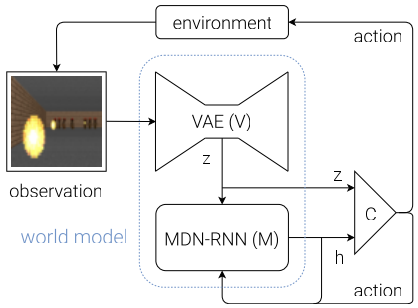
\includegraphics[width=0.7\textwidth,keepaspectratio]{figures/WorldModels.png}
\caption[Flow diagram of the World Models agent's model]{Flow diagram of the agent's model \protect\cite{Algo.WorldModels}. The raw observation is first processed by the Vision at each time step $t$ to produce $z_t$. The input into the Controller is this latent vector $z_t$ concatenated with the Memory hidden state $h_t$ at each time step. The Controller will then output an action vector $a_t$ and will affect the environment. The Memory will then take the current $z_t$ and action $a_t$ as an input to update its own hidden state to produce $h_{t+1}$ to be used at time step $t + 1$.}
\label{Fig.WorldModels}
\end{figure}

The environment provides the agent with a high dimensional visual observation, a game frame, at each time step. The essential task of the Vision model is to encode this high dimensional observation into a low dimensional latent state. To do this, Vision is implemented as Variational Autoencoder \cite{Algo.VAE}. It is trained in an unsupervised manner on randomly generated experience from the environment. The authors assume that the random agent can efficiently explore environment and no iterative training procedure is implemented. The dataset is gathered once and fixed for Vision and Memory training.

Since many complex environment are partially observable, the visual observation at each time step, and hence the latent state, doesn't include full information about the current situation in the environment. To acquire full knowledge, the agent needs to encode what happens over time. This is the role of the Memory. It is implemented as popular recurrent neural network (RNN) architecture called Long Short-Term Memory \cite{Algo.LSTM} and trained on the same data as Vision to predict the next step future latent state that Vision is expected to produce. Because many environments are stochastic in nature, the RNN is trained to output a probability density of the next latent state approximated as a mixture of Gaussian distribution - in literature, this approach is known as Mixture Density Network combined with a RNN \cite{Algo.MDNRNN} (MDN-RNN). Moreover, using the stochastic Memory the authors are able to train more robust Controller, more on that later. \\
To be more precise, the MDN-RNN will model $p(z_{t+1} | o_{\leqslant t}, a_{\leqslant t}) = p(z_{t+1} | h_t) \prod_{i=1}^t q(z_i | o_i)$, where $h_t = f(h_{t-1}, z_t, a_t)$ is the hidden state of the RNN, $f$, that encodes past information about states and actions from the beginning of the episode until the time step $t$. Furthermore, $o_{t}$, $z_{t}$ and $a_{t}$ are the observation, the latent state and the action at time step $t$ respectively. During sampling they can adjust a temperature parameter $\tau$, that scale mixing coefficients in the MDN, to control model uncertainty \cite{Algo.Sketch-RNN}. They find it useful for training the Controller later on.

The Controller model represents the agent's policy. It is responsible for determining course of actions to take in order to solve a given task. Controller is a simple linear model that maps the concatenated latent state $z_t$ and hidden state $h_t$ at the time step $t$ directly to the action $a_t$ at that time step: $a_t = W[z_t h_t] + b$, where $W$ and $b$ are the weight matrix and bias vector of that model.
The authors deliberately made Controller as simple as possible, and trained it separately from Vision and Memory, so that most of the agent's complexity resides in the world model (V and M). The latter can take the advantage of current advances in deep learning that provide tools to train large models efficiently when well-behaved and differentiable loss function can be defined.
Shift in the agent's complexity towards the world model allows the Controller model to stay small and focus its training on tackling the credit assignment problem in challenging RL tasks. It is trained using evolution strategy, which is rather an unconventional choice that only currently have been considered as a viable alternative to popular RL techniques \cite{Algo.ESRL}.

\editnote{Main contributions or where it's SoTa.}
Their solution is able to solve an OpenAI Gym's CarRacing environment \cite{Code.OpenAIGym}, which is the continuous-control, top-down racing task. It is the first known solution to achieve the score required to solve this task. Nonetheless, because the Controller uses real experience for training counted in millions of episodes, they did not improve sample-efficiency compared to other model-free solutions \cite{Algo.CarRacingA3C}. But, what is really interesting, in the process of training the Memory learns to simulate the original environment. The authors show that the learned Controller can function inside of the imagined environment of CarRacing, that is simulated by the Memory.
In the second experiment, they show that the agent can not only play in the imagination, but also it is able to learn solely from imagined experience, produced by its Memory, and successfully transfer this policy back to the actual environment of VizDoom (see fig.~\ref{Fig.VizDoom}). In the first trials, the Controller learned to exploit imperfect simulations of the Model, which only approximates the true environment dynamics. To mitigate this behaviour, they adjust the temperature parameter of MDN-RNN to control the amount of randomness in the Memory, hence controlling the trade-off between realism and exploitability.
The Controller learns from simulated experience, which means that only tens of thousands of episodes from the environment are needed for the training of Vision and Memory. Assuming that each episode consists of hundreds of frames, millions of frames in total are required for training. It makes World Models very sample efficient compared to other state-of-the-art model-free methods that require even two orders of magnitude more data \cite{Algo.A3C}.

\begin{figure}[H]
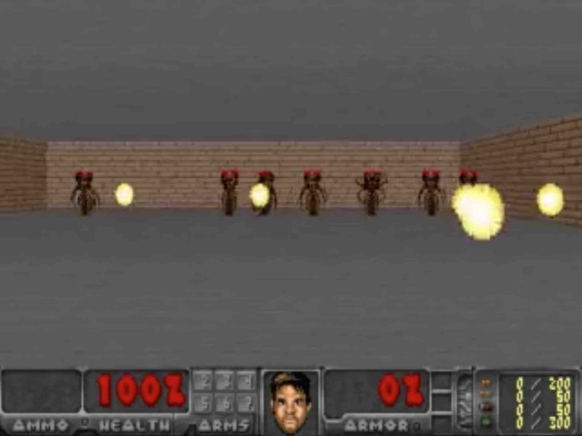
\includegraphics[width=0.7\textwidth,keepaspectratio]{figures/VizDoom.png}
\caption[VizDoom]{VizDoom: the agent must learn to avoid fireballs shot by monsters from the other side of the room with the sole intent of killing the agent \protect\cite{Algo.WorldModels}.}
\label{Fig.VizDoom}
\end{figure}

\editnote{Argument why and how (or not) you base on this work.}
The authors results indicate that their world model is able to model complex environments from visual observations and it can be used for planning. Therefore, it may prove useful for the topic of this thesis.

\subsection{Learning Latent Dynamics for Planning from Pixels}

\editnote{High-level idea or abstract.}
The authors propose the Deep Planning Network \cite{Algo.PlaNet} (PlaNet), a purely model-based agent that learns the environment dynamics from images and chooses actions through fast online planning in latent space. To achieve high performance, the dynamics model must accurately predict the rewards ahead for multiple time steps. They approach this using a latent dynamics model with both deterministic and stochastic transition components. Moreover, they propose a multi-step variational inference objective named latent overshooting.

\editnote{Recurrent state space model}
PlaNet learns a transition model $p(s_t | s_{t-1}, a_{t-1})$, observation model $p(o_t | s_t)$, and reward model $p(r_t | s_t)$ from previously experienced episodes. All of them are Gaussians parameterised by neural networks. The observation model provides a rich training signal but is not used for planning. It also learns an encoder $q(s_t | o_{\leqslant t}, a_{< t})$ to infer an approximate belief over the current hidden state from the history using filtering. This model can be thought of as a non-linear Kalman filter or sequential VAE. The transition model consists of both stochastic and deterministic paths as experiments show that these are crucial for successful planning. \\
Despite its generality, the purely stochastic transitions make it difficult for the transition model to reliably remember information for multiple time steps. In theory, this model could learn to set the variance to zero for some state components, but the optimization procedure may not find this solution. This motivates including a deterministic sequence of activation vectors $\{h_t\}^T_{t=1}$ that allow the model to access not just the last state but all previous states deterministically. The authors use such a model, shown in fig.\ref{Fig.PlaNetModelDesignes}c, that they name recurrent state-space model (RSSM). Intuitively, one can understand this model as splitting the state into a stochastic part $s_t$ and a deterministic part $h_t$, which depend on the stochastic and deterministic parts at the previous time step through the recurrent neural network (RNN). Importantly, all information about the observations must pass through the sampling step of the encoder to avoid a deterministic shortcut from inputs to reconstructions.

\begin{figure}[H]
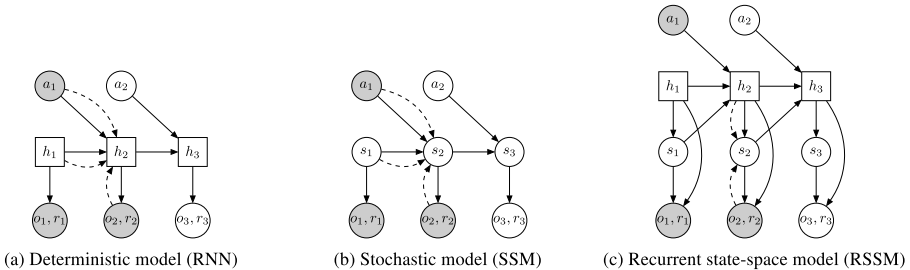
\includegraphics[width=1.0\textwidth,keepaspectratio]{figures/PlaNet/models.png}
\caption[PlaNet latent dynamics model designs]{Latent dynamics model designs \protect\cite{Algo.PlaNet}. In this example, the model observes the first two time steps and predicts the third. Circles represent stochastic variables and squares deterministic variables. Solid lines denote the generative process and dashed lines the inference model. (a) Transitions in a recurrent neural network are purely deterministic. This prevents the model from capturing multiple futures and makes it easy for the planner to exploit inaccuracies. (b) Transitions in a state-space model are purely stochastic. This makes it difficult to remember information over multiple time steps. (c) This model splits the state into stochastic and deterministic parts, allowing the model to robustly learn to predict multiple futures.}
\label{Fig.PlaNetModelDesignes}
\end{figure}

Given these components, the authors implement the policy as a planning algorithm that searches for the best sequence of future actions. In contrast to model-free and hybrid reinforcement learning algorithms, the authors do not use a policy or value network. \\
The cross entropy method \cite{Algo.CEM} (CEM) is used to search for the best action sequence under the model. The authors decided on this algorithm because of its robustness and because it solved all considered tasks when given the true dynamics for planning. CEM is a population-based optimization algorithm that infers a distribution over action sequences that maximize the objective. Starting from zero mean and unit variance time-dependent diagonal Gaussian belief over optimal action sequences up to H, the length of the planning horizon, it repeatedly sample J candidate action sequences, evaluate them under the model, and re-fit the belief to the top K action sequences. After I iterations, the planner returns the mean of the belief for the current time step. Importantly, after receiving the next observation, the belief over action sequences starts from zero mean and unit variance again to avoid local optima. \\
To evaluate a candidate action sequence under the learned model, PlaNet samples a state trajectory starting from the current state belief and sum the mean rewards predicted along the sequence. Since CEM is a population-based optimizer, the authors found it sufficient to consider a single trajectory per action sequence and thus focus the computational budget on evaluating a larger number of different sequences. Because the reward is modeled as a function of the latent state, the planner can operate purely in latent space without generating images, which allows for fast evaluation of large batches of action sequences.

Since the agent may not initially visit all parts of the environment, it needs to iteratively collect new experience and refine the dynamics model. It does so by planning with the partially trained model. Starting from a small amount of S seed episodes collected under random actions, the authors train the model and add one additional episode to the data set every C update steps.

\editnote{Latent overshooting}
Typical variational bound for learning and inference in latent sequence models, as show in fig.\ref{Fig.PlaNetModelUnrolling}a, contains reconstruction terms for the observations and KL-divergence regularisers for the approximate posteriors. A limitation of this objective is that the stochastic path of the transition function $p(s_t | s_{t-1}, a_{t-1})$ is only trained via the KL-divergence regularisers for one-step predictions: the gradient flows through $p(s_t | s_{t-1}, a_{t-1})$ directly into $q(s_{t−1})$ but never traverses a chain of multiple $p(s_t | s_{t-1}, a_{t-1})$. If one could train a model to make perfect one-step predictions, it would also make perfect multi-step predictions, so this would not be a problem. However, when using a model with limited capacity and restricted distributional family, training the model only on one-step predictions until convergence does in general not coincide with the model that is best at multi-step predictions. For successful planning, accurate multi-step predictions are needed. \\
The authors generalize the standard variational bound to latent overshooting, as show in fig.\ref{Fig.PlaNetModelUnrolling}c, which trains all multi-step predictions in latent space. Using only terms in latent space results in a fast regulariser that can improve long-term predictions, it encourages consistency between one-step and multi-step predictions, and is compatible with any latent sequence model. \\
The authors found that several dynamics models benefit from latent overshooting, although their final agent using the RSSM model does not require it.

\begin{figure}[H]
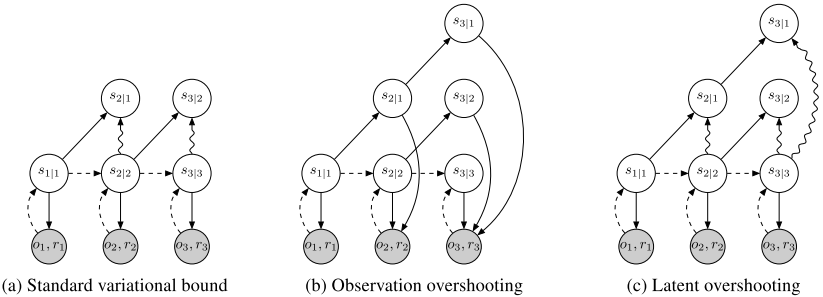
\includegraphics[width=1.0\textwidth,keepaspectratio]{figures/PlaNet/overshooting.png}
\caption[PlaNet latent dynamics model unrolling schemes]{Unrolling schemes \protect\cite{Algo.PlaNet}. The labels $s_{i|j}$ are short for the state at time $i$ conditioned on observations up to time $j$. Arrows pointing at shaded circles indicate log-likelihood loss terms. Wavy arrows indicate KL-divergence loss terms. (a) The standard variational objectives decodes the posterior at every step to compute the reconstruction loss. It also places a KL on the prior and posterior at every step, which trains the transition function for one-step predictions. (b) Observation overshooting decodes all multi-step predictions to apply additional reconstruction losses. This is typically too expensive in image domains. (c) Latent overshooting predicts all multi-step priors. These state beliefs are trained towards their corresponding posteriors in latent space to encourage accurate multi-step predictions.}
\label{Fig.PlaNetModelUnrolling}
\end{figure}

\editnote{Main contributions or where it's SoTa}
Using only pixel observations, PlaNet's agent solves continuous control tasks from DeepMind control suite (see fig.\ref{Fig.DeepMindControlSuite}) with contact dynamics, partial observability, and sparse rewards, which exceed the difficulty of tasks that were previously solved by planning with learned models. PlaNet uses substantially fewer episodes and reaches final performance close to and sometimes higher than strong model-free algorithms.

\begin{figure}[H]
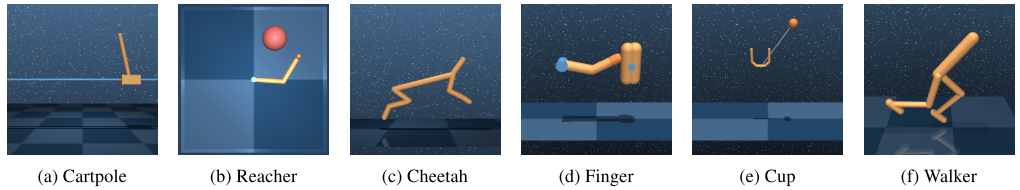
\includegraphics[width=1.0\textwidth,keepaspectratio]{figures/PlaNet/benchmarks.png}
\caption[DeepMind Control Suite]{DeepMind Control Suite: image-based control domains used in PlaNet's experiments \protect\cite{Algo.PlaNet}.}
\label{Fig.DeepMindControlSuite}
\end{figure}

Within 100 episodes, PlaNet outperforms the policy-gradient method A3C \cite{Algo.A3C} trained from proprioceptive states for 100,000 episodes, on all tasks. After 500 episodes, it achieves performance similar to D4PG \cite{Algo.D4PG}, trained from images for 100,000 episodes, except for the finger task. PlaNet surpasses the final performance of D4PG with a relative improvement of 26\% on the cheetah running task.

Moreover, the authors trained a single agent on all six tasks. The agent is not told which task it is facing, it needs to infer this from the image observations. The agent solves all tasks while learning slower compared to individually trained agents. This indicates that the model can learn to predict multiple domains, regardless of the conceptually different visuals.

\editnote{Argument why and how (or not) you base on this work.}
PlaNet is a working example of a model-based agent that learns a latent dynamics model from high-dimensional image observations and chooses actions by fast planning in latent space. The authors show that their agent succeeds at several continuous control tasks from image observations, reaching performance that is comparable to the best model-free algorithms while using 200 times fewer episodes and similar or less computation time. The results show that learning latent dynamics models for planning in image domains is a promising approach. This thesis will adopt PlaNet to its objectives.

\subsection{Model-Based Reinforcement Learning for Atari}

\editnote{High-level idea or abstract.}

\editnote{Main contributions or where it's SoTa.}

\editnote{Argument why and how (or not) you base on this work.}
This is similar approach like in World Models. The authors train the dynamics model and use it to generate new experience, the same as in World Models, but in observations space, opposite to World Models. What this works tries to accomplish is fundamentally different. The main goal is to train good transitions model in the latent states to enable fast simulation. 

\subsection{Value Prediction Network}

\editnote{High-level idea or abstract.}

\editnote{Main contributions or where it's SoTa.}

\editnote{Argument why and how (or not) you base on this work.}
It is model-free/model-based hybrid that learns abstract reward model. It is also not that sample-efficient. It is not quite what this work tries to achieve. This work aim to train fast generative latent dynamics model for efficient simulations and search.

\subsection{A general reinforcement learning algorithm that masters chess, shogi, and Go through self-play}

\editnote{High-level idea or abstract.}

\editnote{Main contributions or where it's SoTa.}

\editnote{Argument why and how (or not) you base on this work.}
State-of-the-art general search algorithm, that requires model dynamics. Goal would be to enable it to work with the learned model.

\subsection{Recurrent Environment Simulators}

\editnote{High-level idea or abstract.}

\editnote{Main contributions or where it's SoTa.}

\editnote{Argument why and how (or not) you base on this work.}
The authors train efficient environment simulators. To make them efficient, they train dynamics model in latent state-space. This thesis takes from this idea and expand it to planning using learned model.

\subsection{Learning and Querying Fast Generative Models for Reinforcement Learning}

\editnote{High-level idea or abstract.}

\editnote{Main contributions or where it's SoTa.}

\editnote{Argument why and how (or not) you base on this work.}
The authors further explores topic of fast generative models that could be used in model-based reinforcement learning. Their ideas find application in this thesis solution.
